\documentclass[conference]{IEEEtran}
\IEEEoverridecommandlockouts
% The preceding line is only needed to identify funding in the first footnote. If that is unneeded, please comment it out.
\usepackage{cite}
\usepackage{amsmath,amssymb,amsfonts}
\usepackage{algorithmic}
\usepackage{graphicx}
\usepackage{textcomp}
\usepackage{xcolor}
\def\BibTeX{{\rm B\kern-.05em{\sc i\kern-.025em b}\kern-.08em
    T\kern-.1667em\lower.7ex\hbox{E}\kern-.125emX}}
\begin{document}

\title{Menganalisis Kekuatan Sinyal Wifi Menggunakan inSSIDer\\

}

\author{\IEEEauthorblockN{Kevin Antony K}
\IEEEauthorblockA{\textit{Fakukultas Teknologi Informasi} \\
\textit{Institut Teknologi Batam}\\
Batam, Indonesia \\
1922003@student.iteba.ac.id}


}

\maketitle

\begin{abstract}
    Kemajuan teknologi informasi pada saat ini terus berkembang seiring dengan kebutuhan manusia yang menginginkan kemudahan, kecepatan, dan keakuratan dalam memperoleh informasi.
    Oleh karena itu kemajuan teknologi informasi di bidang transmisi pada saat ini yang berkembang selain fiber optic ialah penggunaan perangkat wireless.
    Perangkat wireless ini memungkinkan adanya hubungan para pengguna informasi dalam melakukan aktivitasnya.
 
\end{abstract}


\section{Pendahuluan}

\subsection{Latar Belakang}
Kemajuan teknologi informasi pada saat ini terus berkembang seiring dengan kebutuhan manusia yang menginginkan kemudahan, kecepatan, dan keakuratan dalam memperoleh informasi. 
Oleh karena itu kemajuan teknologi informasi khususnya dibidang teknologi jaringan nirkabel atau sering kita kenal dengan Wireless.
\vspace{1pt}

Perangkat ini juga menjadi kebutuhan utama dimasa pandemi dimana semua aktivitas dilakukan dirumah saja.Perangkat wireless ini memungkinkan adanya hubungan para pengguna informasi dalam melakukan aktivitasnya.
Teknologi ini berkembang cukup pesat terutama di bidang jaringan komunikasi dimana karena sifatnya yang fleksibel 
membuatnya lebih hemat dalam beberapa aspek.

\section{Pembahasan}

\subsection{Pengertian Wireless Networking}
Wireless Network (jaringan nirkabel) adalah bidang disiplin yang berkaitan dengan komunikasi antar sistem komputer tanpa menggunakan kabel. Jaringan nirkabel ini sering dipakai untuk jaringan komputer baik pada jarak yang dekat (beberapa meter, memakai alat/pemancar bluetooth) maupun pada jarak jauh (lewat satelit). Bidang ini erat hubungannya dengan bidang telekomunikasi, teknologi informasi, dan teknik komputer. Jenis jaringan yang populer dalam kategori jaringan nirkabel ini meliputi: Jaringan kawasan lokal nirkabel (wireless LAN/WLAN), dan Wi-Fi.

Jaringan nirkabel biasanya menghubungkan satu sistem komputer dengan sistem yang lain dengan menggunakan beberapa macam media transmisi tanpa kabel, seperti:gelombang radio, gelombang mikro, maupun cahaya infra merah.

\subsection{Kelebihan dan Kekurangan Wireless Network}
1. Kelebihan Wireless Network
\begin{itemize}
    \item  Pembangunan jaringan yang cepat
    \item  Mudah dan murah untuk direlokasi
    \item  biaya pemeliharaannya murah
    \item  infrastruktur berdimensi kecil dan Mudah Dikembangkan
    \item  sumber-sumber file bisa pindahkan dengan   mudah tanpa menggunakan media kabel.
    \item mudah sekali untuk di-setup dan juga handal sehingga cocok untuk pemakaian di kantor maupun di rumah.
\end{itemize}
\vspace{0.1cm}

2. Kekurangan Wireless Network
\begin{itemize}
    \item Keamanan atau kerahasiaan data-data rentan serta Interferensi gelombang radio.
    \item Delay (kelambatan) yang besar
    \item Biaya peralatan rata-rata mahal
    \item Produk dari produsen yang berbeda-beda kadang tidak kompatibel atau cocok
    \item  Kualitas sinyalnya dipengaruhi oleh keadaan udara maupun cuaca
    \item Mahal dalam investasinya dan  Kemungkinan penyadapan koneksinya lebih besar terjadi, jika dibandingkan dengan menggunakan media kabel.
\end{itemize}

\subsection{Tipe-tipe Wireless Network}
1.Wireless Personal Area Network (WPAN)
WPAN (Wireless Personal Area Network) adalah sebuah bentuk komunikasi wireless yang terbatas hanya pada jarak pendek dan umumnya hanya terbatas untuk dua buah perangkat elektronik.
\vspace{5pt}

2.Wireless Wide Area Network (WWAN)
WWAN adalah sebuah bentuk komunikasi nirkabel yang memiliki area sangat luas, antara lain untuk penggunaan selular seperti 2G, 3G, 4G, dan lain sebagainya
\vspace{5pt}

3.Wireless Local Area Network (WLAN)
WLAN (Wireless Local Area Network) adalah sebuah bentuk komunikasi nirkabel yang memiliki area terbatas seperti dalam suatu ruangan ataupun sebuah gedung. WLAN memiliki standar komunikasi yang diatur oleh sebuah lembaga. Standar komunikasi data yang digunakan dalam WLAN umumnya adalah keluarga Institute of Electrical and Electronics Engineers (IEEE) 802.11.
\begin{itemize}
    \item  IEEE 802.11a bekerja pada frekuensi 5GHz dan mempunyai kecepatan maksimum 54 Mbps.
    \item IEEE 802.11b bekerja pada frekuensi 2,4GHz dan mempunyai kecepatan sampai dengan 11Mbps.
    \item IEEE 802.11g bekerja pada frekuensi yang sama dengan IEEE 802.11b yaitu 2,4GHz, namun memiliki kecepatan maksimal yang lebih besar, yaitu 54Mbps.
    \item   IEEE 802.11n yang bekerja pada dua frekuensi yaitu 2,4 dan 5GHz dengan kecepatan maksimum adalah 100 sampai dengan 210 Mbps
\end{itemize}
\vspace{5pt}

4.Wireless MAN (WMAN)
\vspace{5pt}

5.Cellular Network
\subsection{Perhitungan Kecepatan Internet}
kecepatan akses internet adalah kecepatan transfer data pada saat melakukan akses melalui jalur internet. Kecepatan transfer data adalah jumlah data dalam bit yang melewati suatu media tertentu dalam satu detik.
Jadi kalau ditulis dengan rumus, Kecepatan Internet (transfer data) dapat dihitung dengan rumus:
\vspace{2pt}

Kecepatan=Jumlah file data : Waktu (Sekon)

Jumlah file data = Kecepatan x waktu

\section{Metode pengerjaan dan Langkah-langkah}
1. Metode Pengerjaan
Metode yang digunakan adalah metode Penelitian Kuantitatif yaitu dengan melakukan survei pada semua teori yang menunjang keberhasilan dalam wireless networking dan juga Eksperimen yaitu menggunakan inSSIDer untuk melihat kekuatan sinya dan jarak maksimum sinyal serta hambatan yang diperoleh
\vspace{4pt}

2.Langkah-langkah 
\begin{itemize}
    \item pertama menyiapkan aplikasi inSSIDer
    \item Kemudian mencari wifi yang terhubung atau yang tertangkap pada aplikasi
    \item melakukan conection dengan wifi yang akan kita survei
    \item lakukan pada jarak yang dekat dengan sumber pemancar wifi (router) dan lakukan pada jarak yang jauh dari router
    \item lihat perbedaan yang dihasilkan dari perbandingan jarak
    \item faktor apa saja yang menyebabkan terjadinya Lost conection
    \item Catat semua perubahan sebagai laporan
\end{itemize}
\vspace{4cm}

\begin{figure}[h]
\centering
    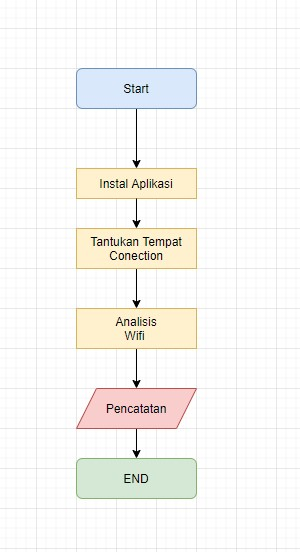
\includegraphics[width=.4\textwidth]{image/001.jpg}
     \caption{Flowchart Langkah-langkah}
\end{figure}

\section{Hasil}
\subsection{Apa itu inSSIDer}
inSSIDer adalah software yang berguna untuk memindai jaringan dalam jangkauan antena Wi-Fi komputer Anda, melacak kekuatan sinyal dari waktu ke waktu, dan menentukan pengaturan keamanan mereka (termasuk apakah atau tidak mereka dilindungi oleh password). inSSIDer, di sisi lain, bekerja dengan mempesona pada kedua Vista dan XP, dan ini open-source untuk boot. Access Point adalah sebuah perangkat jaringan yang berisi sebuah transceiver dan antena untuk transmisi dan menerima sinyal ke dan dari clients remote. Dengan access points (AP) clients wireless bisa dengan cepat dan mudah untuk terhubung kepada jaringan LAN kabel secara wireless. Ini harus dimiliki untuk memburu jaringan Wi-Fi di jalan bebas, untuk Windows, membutuhkan .NET 2.0. Pengguna Mac, cek iStumbler. InSSIDer adalah aplikasi GRATIS, open-source Wi-Fi scanning software. Untuk lebih jelasnya klik dij artikel inSSIDer.

\subsection{Frekuensi 2.4GHz dan 5.0GHz}
Sebelum kita mengunakan inSSIDer kita perlu mengetahui apa perbedaan sinyal atau frekuensi dari 2.4 dan 5.0 GHz ini seperti apa 
\vspace{2pt}

\begin{itemize}
    \item Perbedaan Frekuensi 2.4GHz dan 5GHz
    \vspace{2pt}
    
Frekuensi 2.4 GHZ memiliki beberapa ciri yang sangat jelas terlihat yaitu bekerja dengan 3 channel tanpa overlapping, standar wireless adalah B, G dan N, jangkauan jaringan yang lebih luas, dan tingkat gangguan yang lebih tinggi. Sementara itu frekuensi 5 GHz memiliki sekitar 23 channel non over lapping, dengan standar jaringan A, N dan AC, jangkauan yang lebih kecil dan gangguan yang lebih sedikit dibandingkan dengan frekuensi 2.4GHz.
\begin{figure}[h]
\centering
    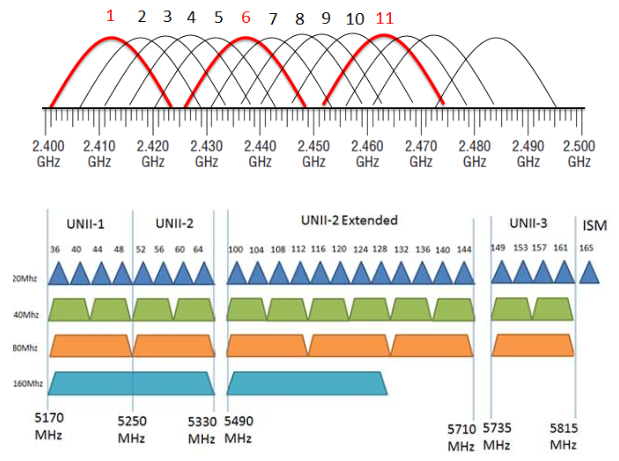
\includegraphics[width=.4\textwidth]{image/002.png}
     \caption{https://blog.dhanipro.com/artikel/teknologi/perbedaan-frekuensi-24-ghz-dan-5-ghz-c1eee1}
\end{figure}

\item Kecepatan Jaringan Frekuensi 2.4GHz dan 5GHz
\vspace{2pt}

Pada dasarnya standar GHz sama sekali tidak memberikan pengukuran yang jelas untuk kecepatan maksimum yang bisa didapatkan dari jaringan nirkabel. Sebuah perangkat nirkabel yang bekerja untuk frekuensi 5 GHz juga bisa mencapai kecepatan data hingga 54 Mbps, kecepatan ini juga bekerja untuk frekuensi 2.4 GHz. Namun kedua frekuensi ini juga harus diatur sesuai dengan tingkat pemakaian pada lingkungan khusus.
\item Tingkat Gangguan
\vspace{2pt}

Tingkat Gangguan dari frekuensi 5 GHz memang lebih kecil dibandingkan dengan tingkat gangguan yang sering muncul pada frekuensi 2.4 GHz. Hal ini bisa terjadi karena ada beberapa perangkat elektronik dan komunikasi lain yang memang memakai tingkat frekuensi 2.4 GHz. Frekuensi 2.4 GHz juga bisa ditemukan untuk jaringan telepon, microwave, komputer dan perangkat lain. Jadi pemakai WiFi dengan frekuensi 2.4 GHz harus berusaha untuk mengurangi beberapa gangguan lingkungan yang terjadi karena tabrakan jaringan.
\item Jangkauan Jaringan
\vspace{2pt}

Jangkauan untuk 5 GHz memang lebih pendek dibandingkan dengan jangkauan yang bekerja untuk frekuensi 2.4 GHz. Untuk memilih jaringan yang akan dipakai tentu Anda harus memilih daya jangkauan yang diinginkan. Hukumnya adalah semakin tinggi frekuensi maka daya jangkauan akan lebih kecil, sebaliknya semakin rendah frekuensi maka daya jangkauan akan lebih panjang atau jauh dengan asumsi kedua frekuensi 2,4 GHz dan 5 GHz diukur dengan daya(power) yang sama. Sifat frekuensi J.Maxwell

\begin{figure}[h]
\centering
    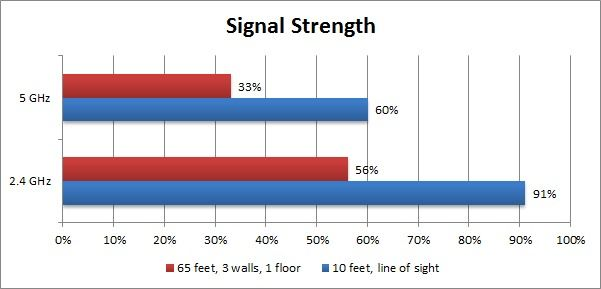
\includegraphics[width=.4\textwidth]{image/003.jpg}
     \caption{https://blog.dhanipro.com/artikel/teknologi/perbedaan-frekuensi-24-ghz-dan-5-ghz-c1eee1}
\end{figure}

\item Tingkat Pemakaian
\vspace{2pt}

Pemakaian frekuensi 2.4 GHz dan 5 Ghz harus disesuaikan dengan daya pemakaian yang diinginkan. Beberapa tujuan yang paling sesuai untuk 2.4 GHz adalah untuk akses internet sederhana seperti pencarian data, browsing dan penggunakan email saja karena beberapa aplikasi ini memang tidak banyak mengambil bandwith dan bisa bekerja dengan baik meskipun memiliki daya jangkau jarak yang lebih luas. Namun jika Anda ingin memakai jaringan untuk keperluan yang lebih khusus dan membutuhkan tingkat keamanan khusus maka bisa memilih frekuensi 5.8 GHz yang memiliki daya jangkau jarak yang lebih pendek.
\end{itemize}
\subsection{Instalasi dan Penggunaan inSSIDer}
\begin{itemize}
    \item instal aplikasi inSSIDer dan login 
    \begin{figure}[h]
\centering
    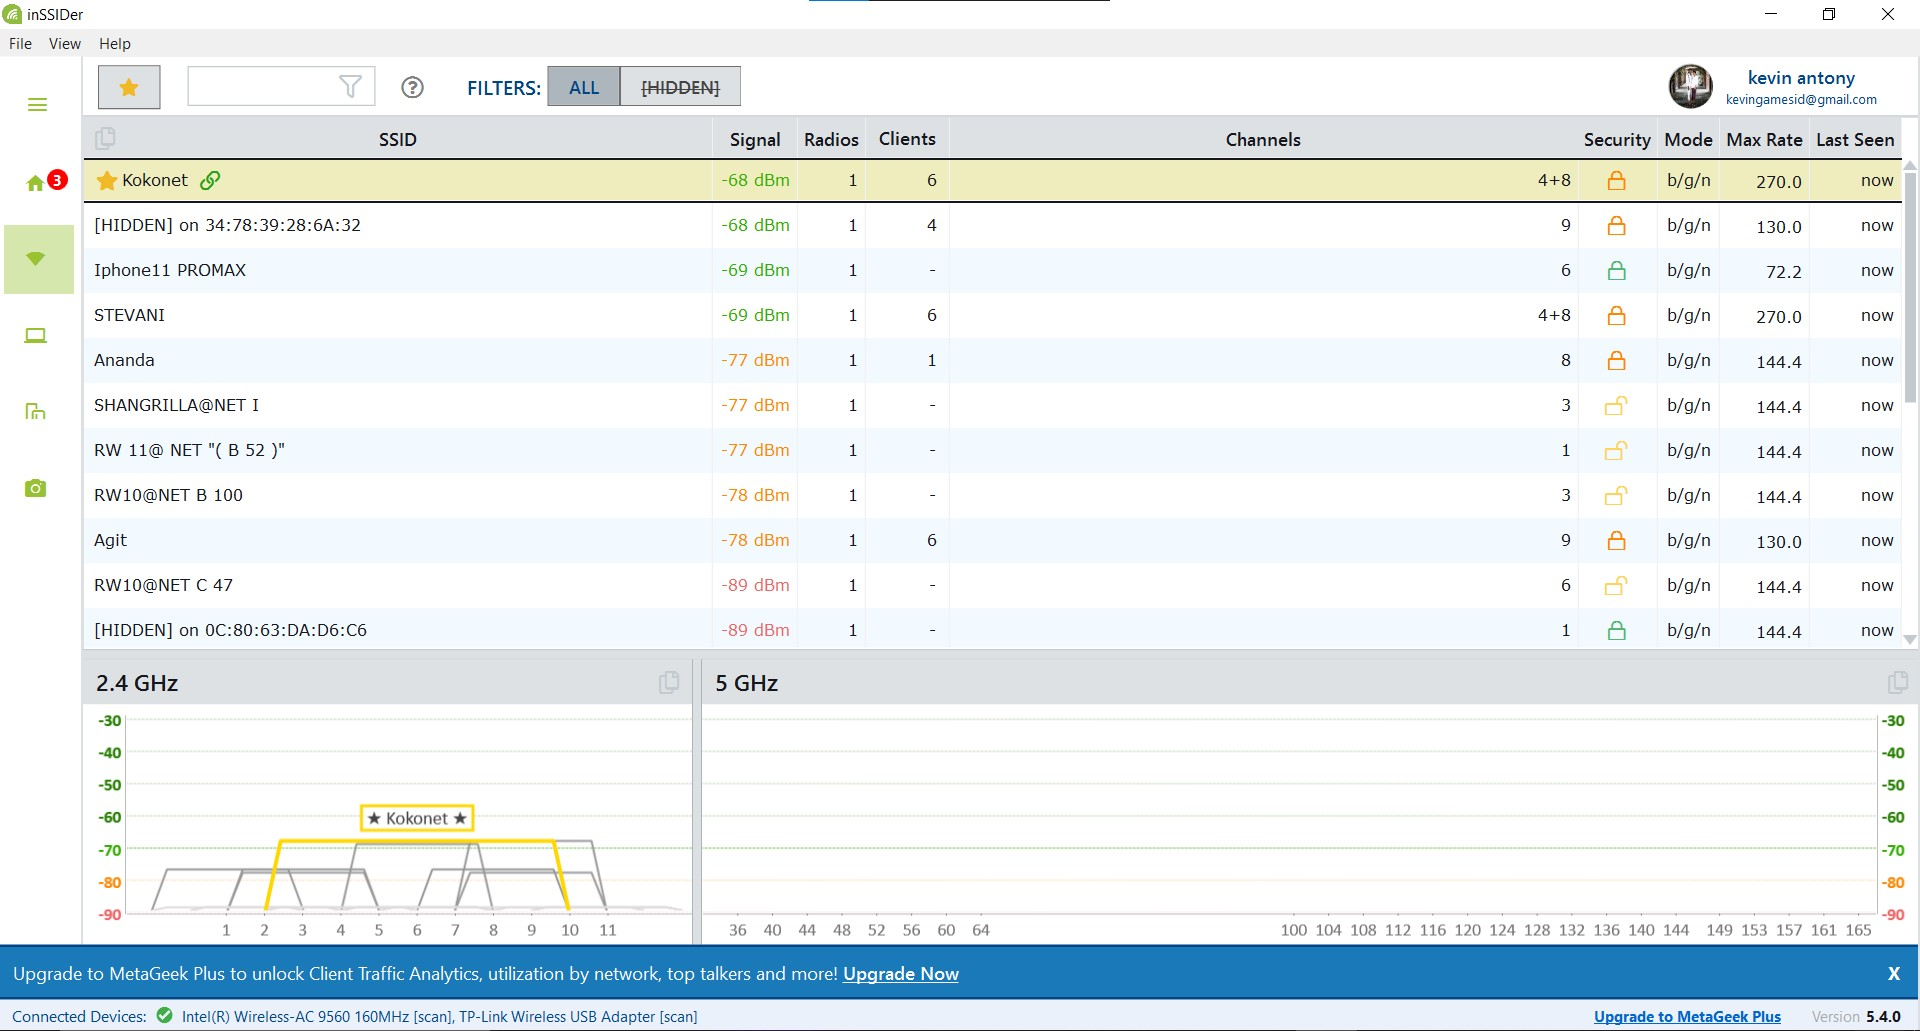
\includegraphics[width=.4\textwidth]{image/004.jpg}
     \caption{Tampilan setelah login ke inSSIDer}
     \end{figure}
     \item setelah sudah masuk Terlihat bagian-bagian 
penting seperti filter, network list, network information, serta spektrum sinyal dalam bentuk grafik.kita bisa lihat semua wifi yang terbaca frekuensinya oleh wifi adapter yang ada di laptop atau pc kita
\vspace{2cm}

\item kemudian kita lihat wifi yang yang terhubung atau conection dengan laptop kita dengan lambang rantai hijau 
    \begin{figure}[h]
\centering
    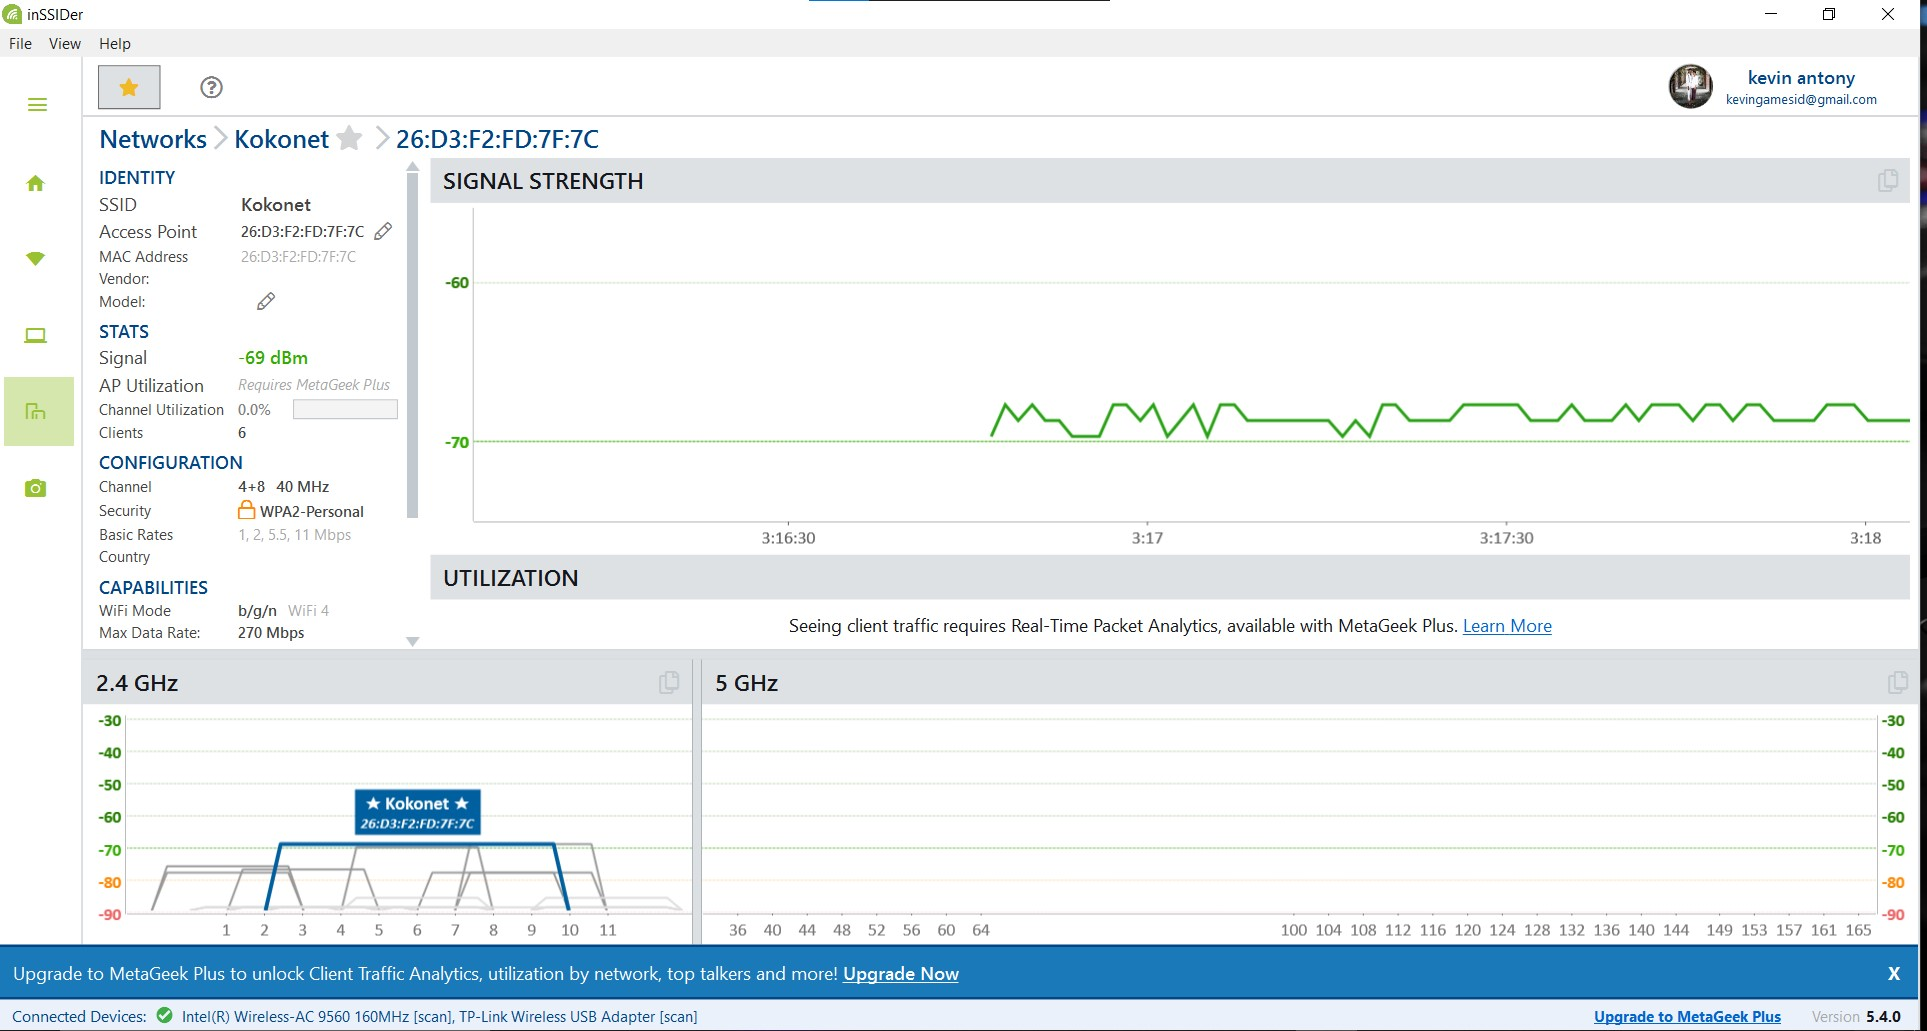
\includegraphics[width=.4\textwidth]{image/005.jpg}
     \caption{Tampilan wifi yang Terhubung}
     \end{figure}
\item ini adalah tampilan wifi yang terhubung dengan laptop saya jarak laptop dengan router kira kira 6-7 m karna itu wifi tetangga saya 
\vspace{2pt}

kecepatan yang terbaca = -69dBm 
\vspace{1pt}

Frekuensinya = 2.4 GHz
\vspace{1pt}

Max Data rate = 270 Mbps
\vspace{1pt}

Penghalang Lost Conection = Tembok dengan tebal 15 cm 3 buah dengan jarak masing masing tembok 3 - 4 meter sebagai penghalang sinyal 

\item ini adalah tampilan ketika saya hanya berjarak 2 meter dengan router dengan penghalan dinding dengan ketebalan 30 cm
\vspace{2pt}

kecepatan yang terbaca = -62 - (-56)dBm 
\vspace{1pt}

Frekuensinya = 2.4 GHz
\vspace{1pt}

Max Data rate = 270 Mbps
    \begin{figure}[h]
\centering
    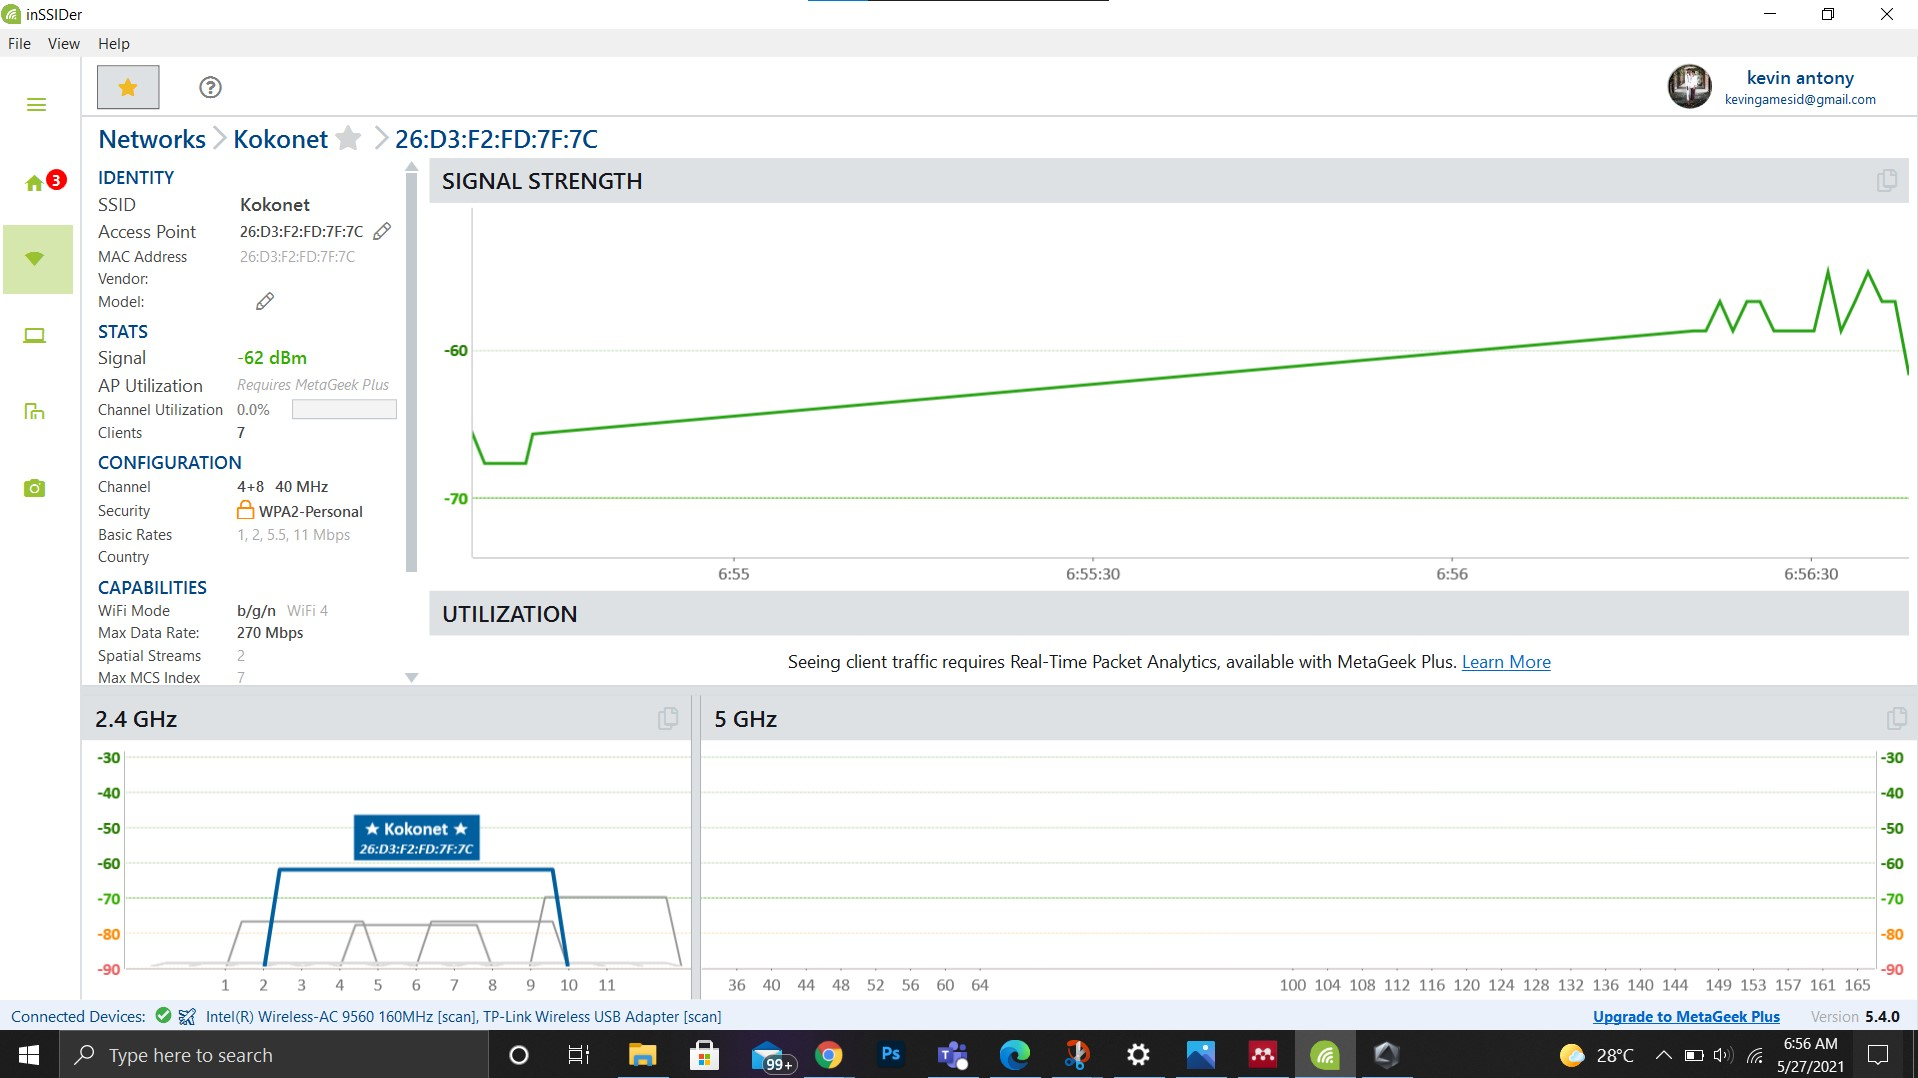
\includegraphics[width=.4\textwidth]{image/007.jpg}
     \caption{Tampilan wifi dengan jarak 2 M}
     \end{figure}
\item ketika jarak 10 meter dengan penghalang 1 buah rumah
    \begin{figure}[h]
\centering
    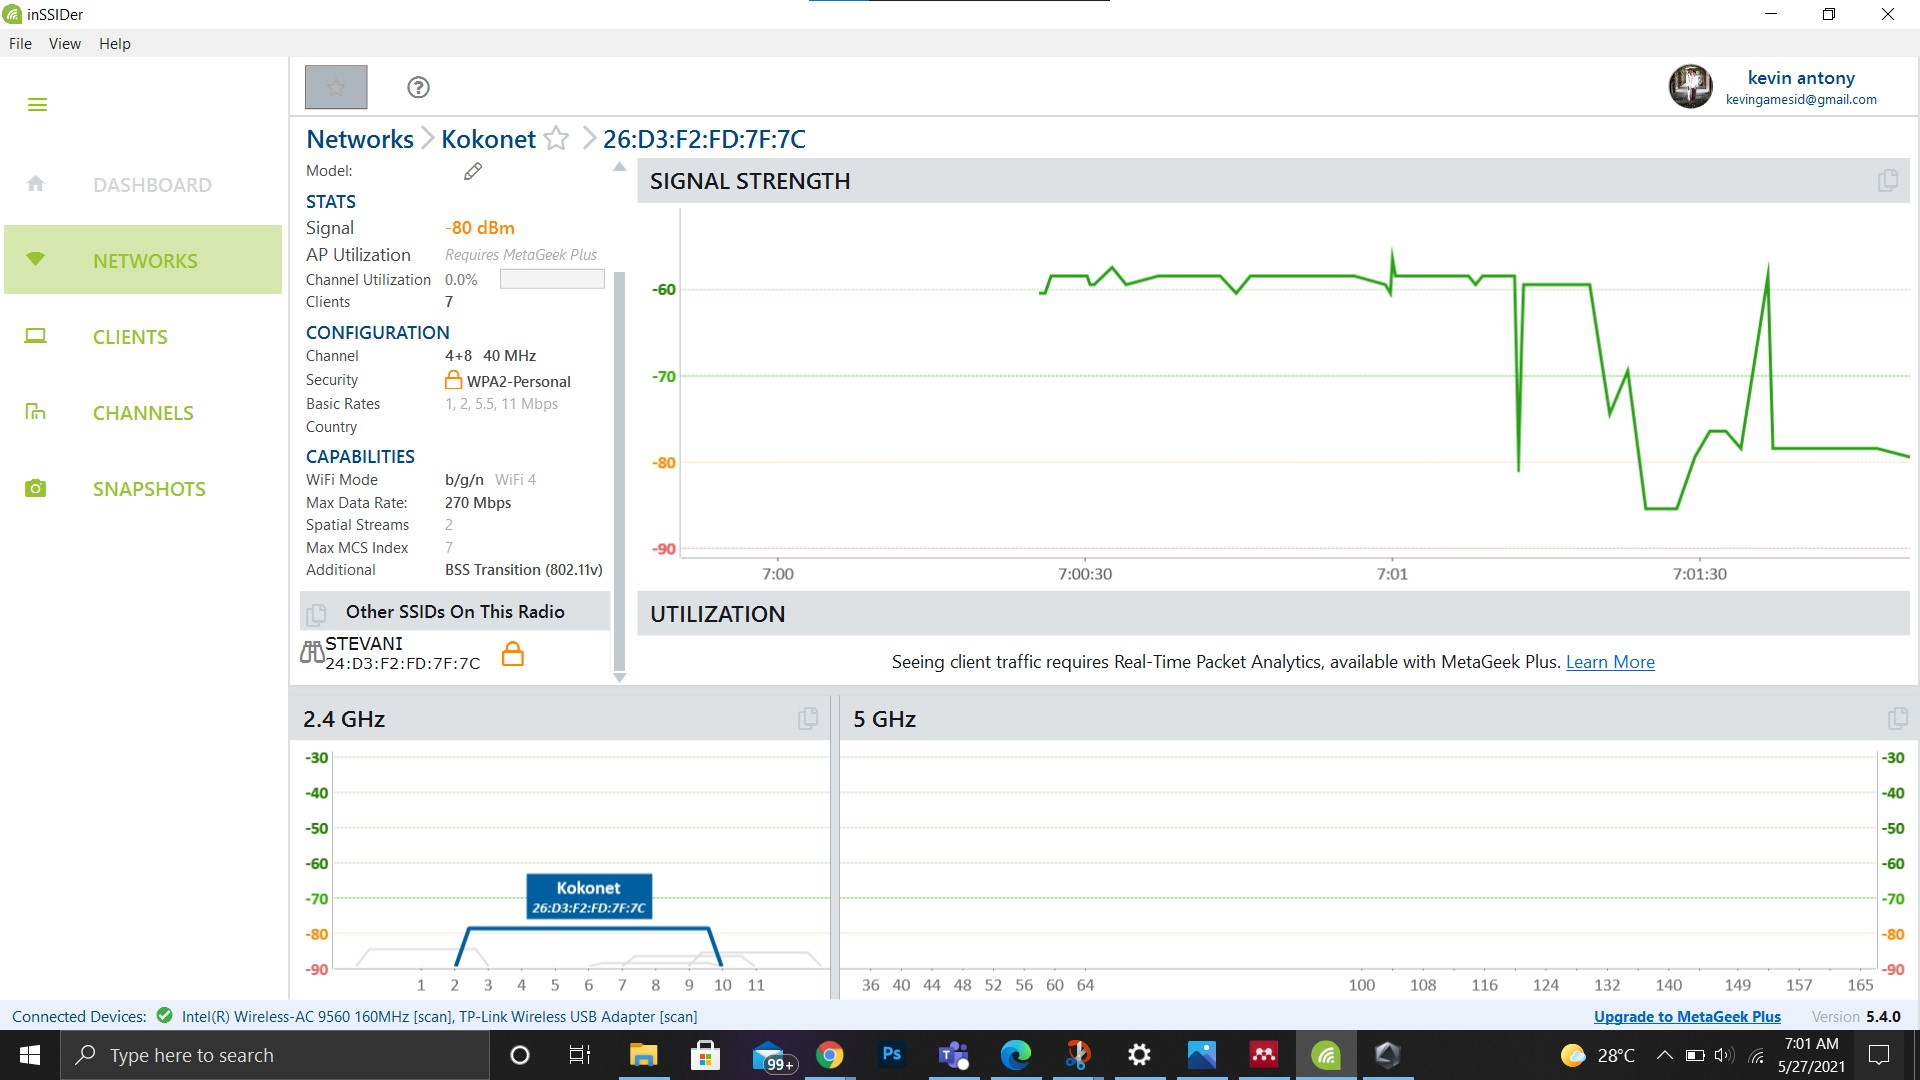
\includegraphics[width=.3\textwidth]{image/008.jpg}
     \caption{Tampilan wifi dengan jarak 10 M}
     \end{figure}
     \vspace{2cm}
     
kecepatan yang terbaca = -78 - (-80)dBm 
\vspace{1pt}

Frekuensinya = 2.4 GHz
\vspace{1pt}

Max Data rate = 270 Mbps
\item ini adalah denah ketika saya keluar rumah dan menetukan jarak maxsimum dari jangkauan frekuensi sinyalnya
    \begin{figure}[h]
\centering
    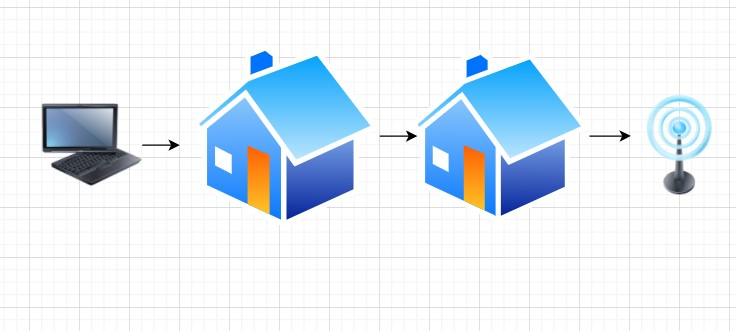
\includegraphics[width=.4\textwidth]{image/006.jpg}
     \caption{Denah conection}
     \end{figure}
\item Jarak 13 meter dari suber sinyal dengan penghalang sesuai denah yaitu 2 buah rumah
\vspace{2pt}

kecepatan yang terbaca = -85 - (-87)dBm dan mulai kurang stabil sinyalnya
\vspace{1pt}

Frekuensinya = 2.4 GHz
\vspace{1pt}

Max Data rate = 270 Mbps
    \begin{figure}[h]
\centering
    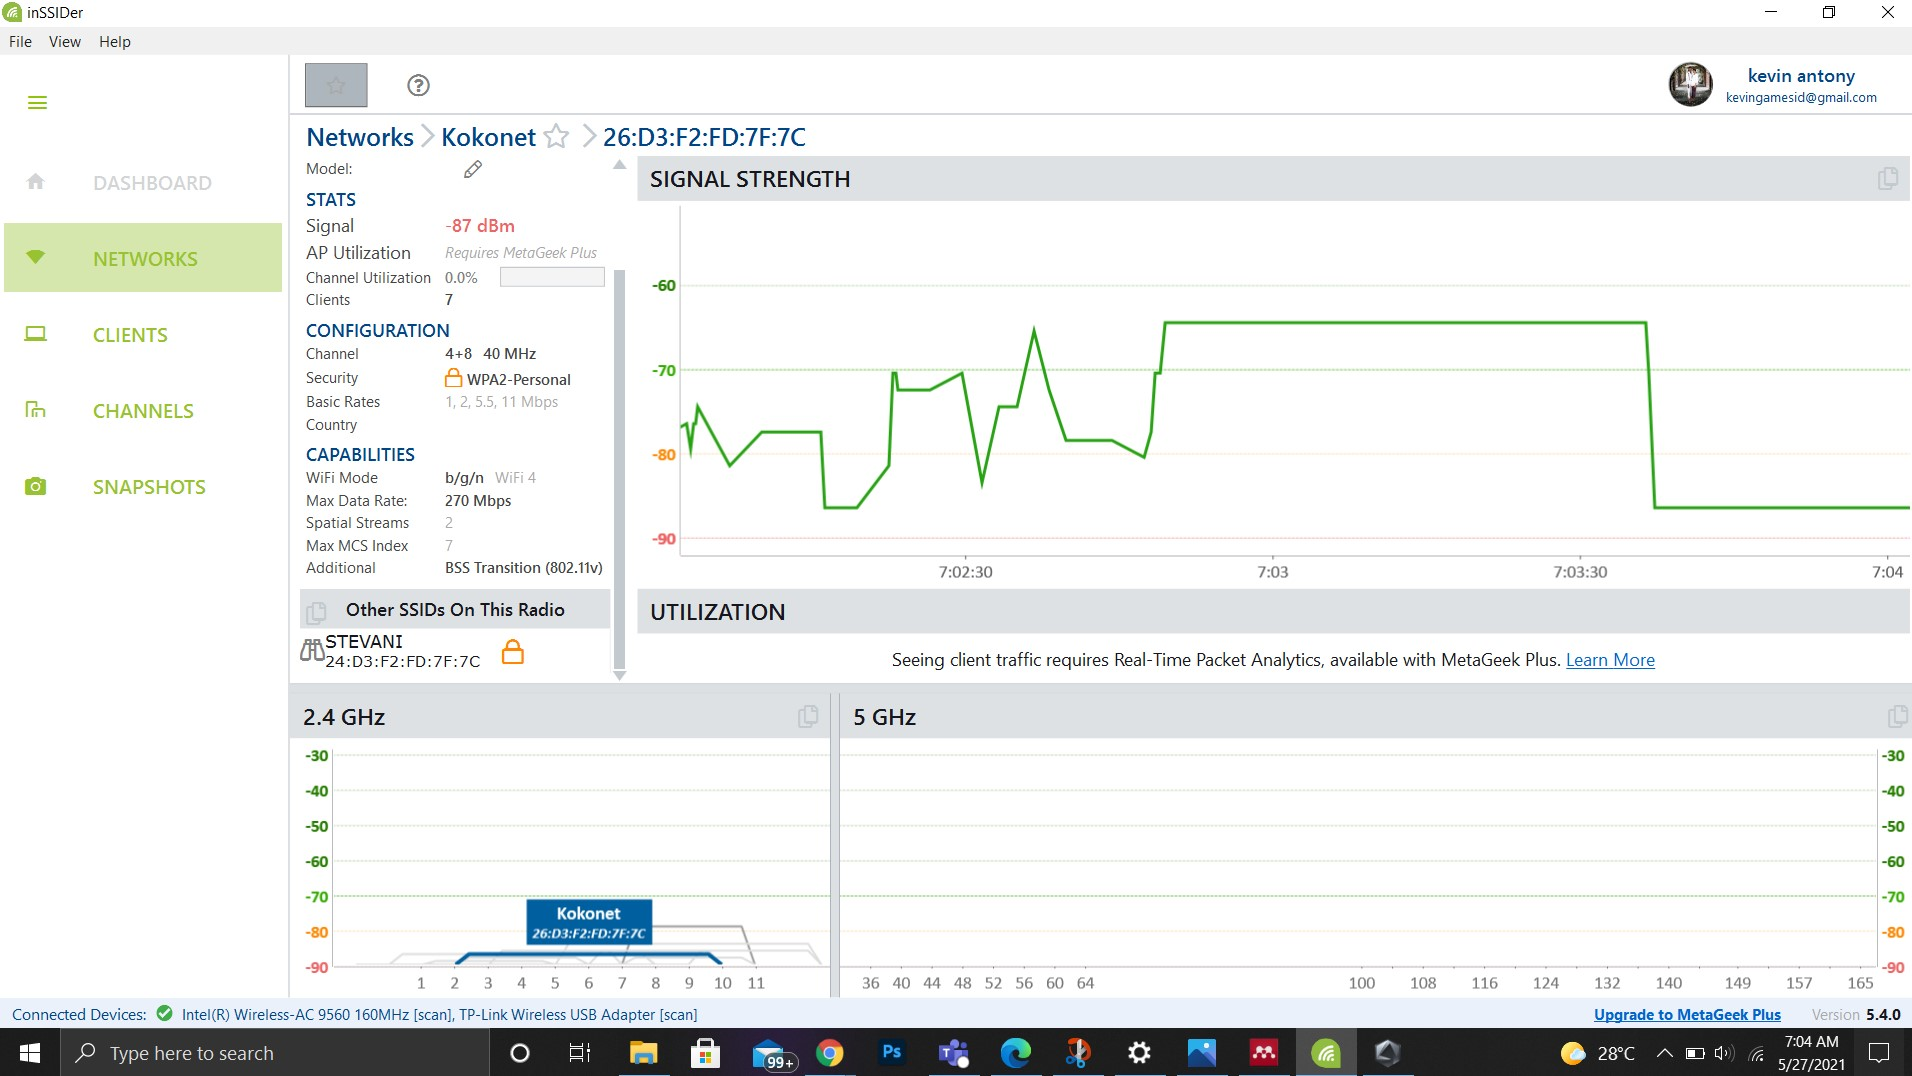
\includegraphics[width=.4\textwidth]{image/009.jpg}
     \caption{jarak 13 M}
     \end{figure}
\item pada jarak 16-18 dengan penghalang yang sama 2 rumah dan permukaan sedikit menurun 
\vspace{2pt}

kecepatan yang terbaca = -87 dBm dan mulai kurang stabil sinyalnya kadang kembali ke -85 dBm
\vspace{1pt}

Frekuensinya = 2.4 GHz
\vspace{1pt}

Max Data rate = 270 Mbps
    \begin{figure}[h]
\centering
    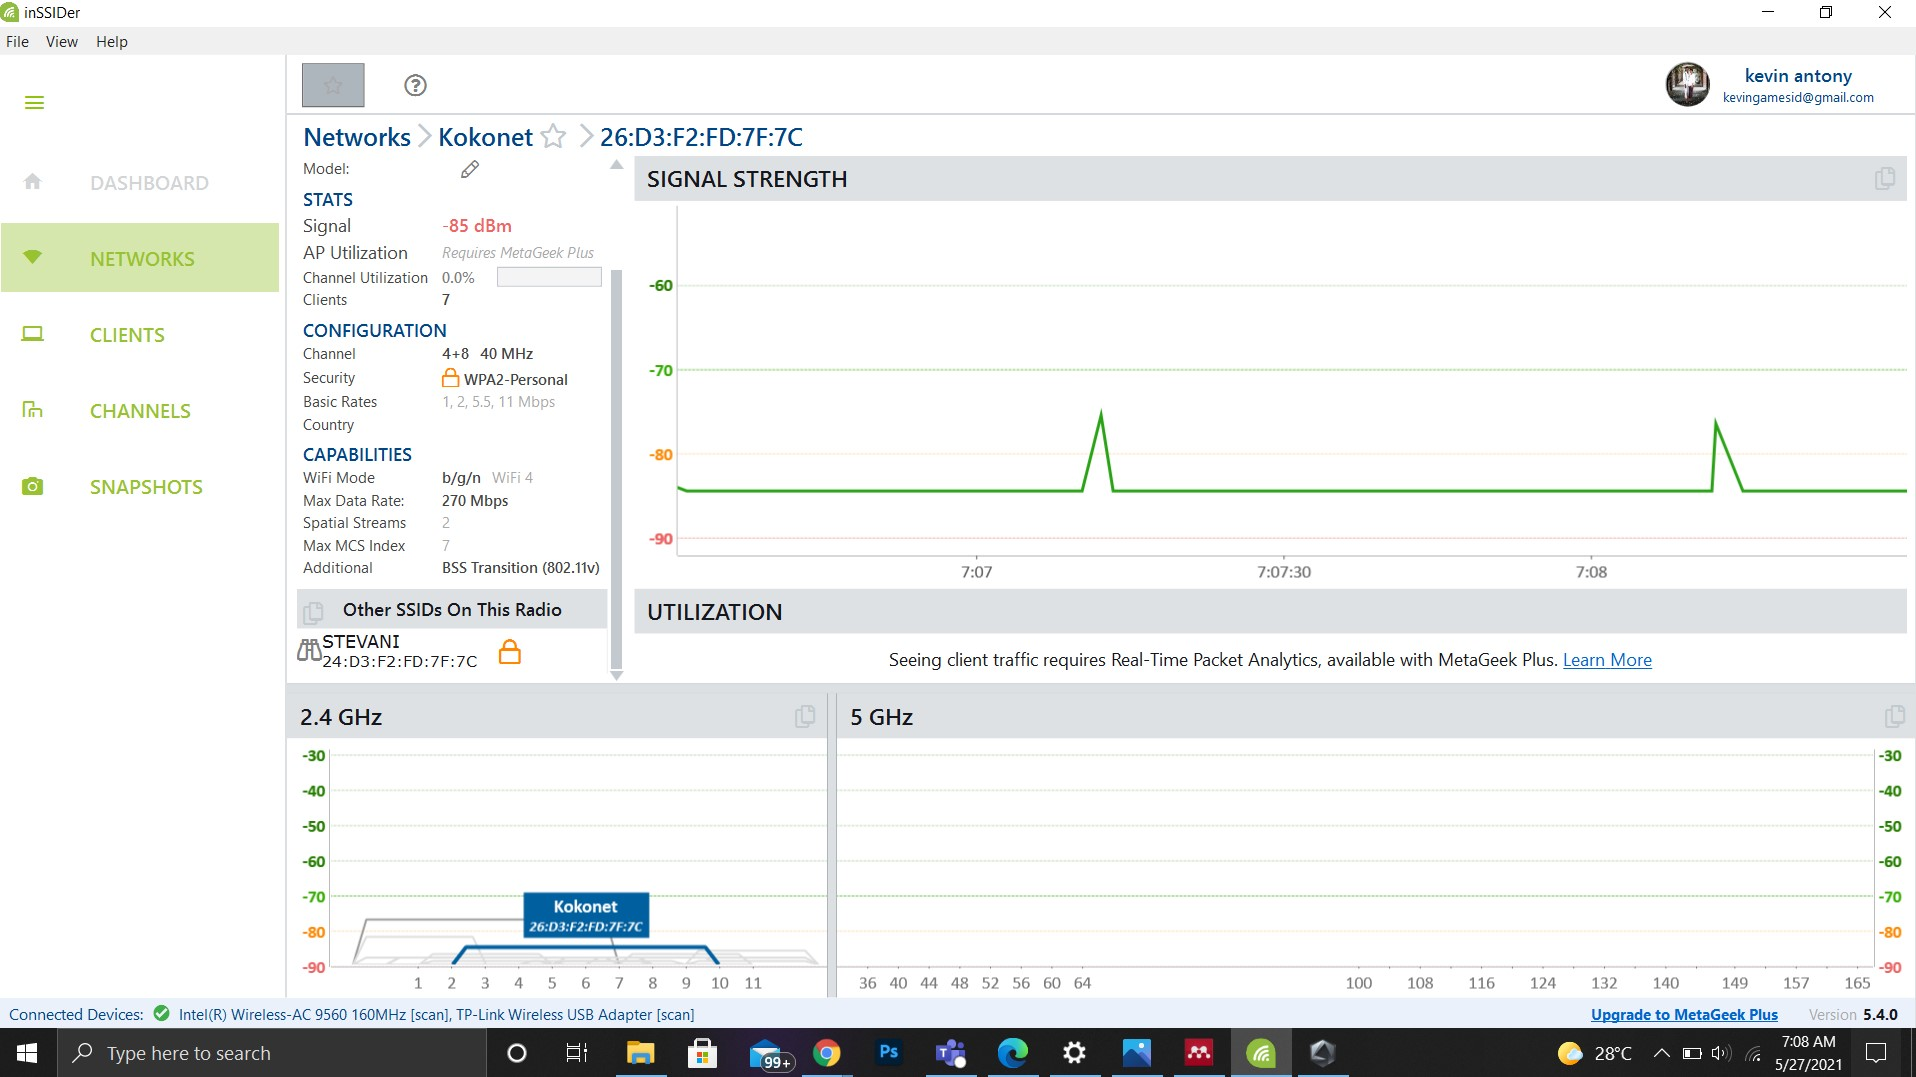
\includegraphics[width=.4\textwidth]{image/010.jpg}
     \caption{jarak 18 M}
     \end{figure}
     \vspace{2cm}

\item ini jarak maksimum yang bisa diperoleh dari pemancar sinya wifi ini dengan penghalang 2 buah rumah dan jalan atau permukaan sedikit lebih rendah serta jaraknya sekitar 30 meter
\vspace{2pt}

kecepatan yang terbaca = -87 dBm dan terus turun serta terjadi lost conection
\vspace{1pt}

Frekuensinya = 2.4 GHz
\vspace{1pt}

Max Data rate = 270 Mbps
    \begin{figure}[h]
\centering
    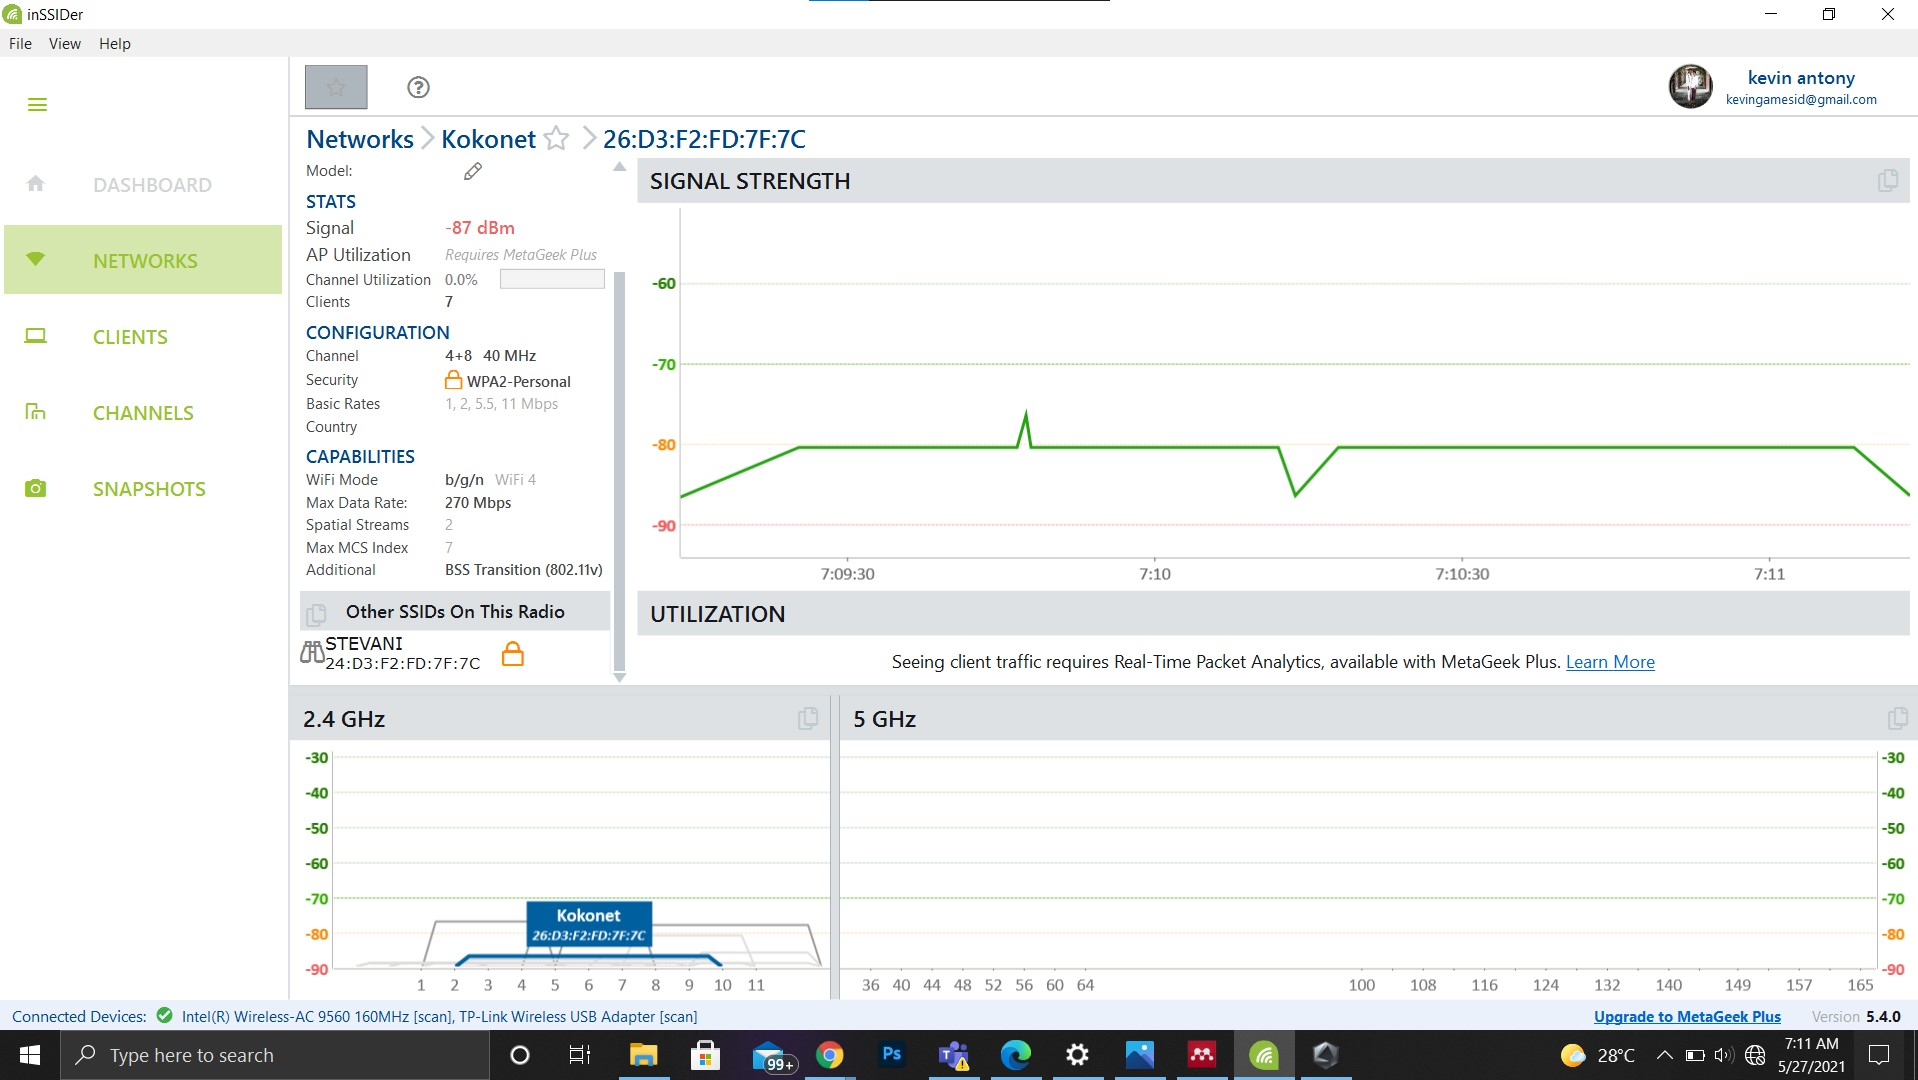
\includegraphics[width=.4\textwidth]{image/011.jpg}
     \caption{jarak 30 M}
     \end{figure}
\end{itemize}
\section{Kesimpulan}
Dari pernelitian dan percobaan yang saya lakukan adalah ketika kita didalam ruangan kemungkinan koneksi tergangu sangat tinggi karna bukan hanya tehalang oleh tembok tetapi juga Flapon rumah dan ketika keluar sinyal cenderung sedikit lebih stabil tetapi disini penghalang juga berpengaruh serta jarak frekuensi yang dapat ditangkap juga menurun bahkan dijarak maksimum terjadi lost konection dan juga dalam hal ini aplikasi inSSIDer menbantu kita untuk memahami grafik dan bisa mengimplementasikan kedalam jarak jangkauan nya.
\vspace{1pt}

Dari hasil Experimen ini kita bisa mengetahui apa yang menjadi prolblem dan penyebab utama dari terjadinya lost control pada sinya wifi dan berapa besar distraction yang ada dari jumlah rumah atau objeck penghalang lainnya yang menyebabkan terjadinya distraction tersebut untuk penggunaan IEEE 802.11 g sekarang tidak banyak dari kita orang awam dapat membedakannya padahal itu adalah yang kita gunakan dan pakai setiap menit bahkan detik untuk trknologi ini sendiri di indonesia sudah mulai banyak jenisnya 
\vspace{1pt}

\subsection{Jenis Jenis Wifi Dan jaringan Yang tersebar atau yang Umum Di Kalangan Masyarakat}
\begin{figure}[h]
\centering
    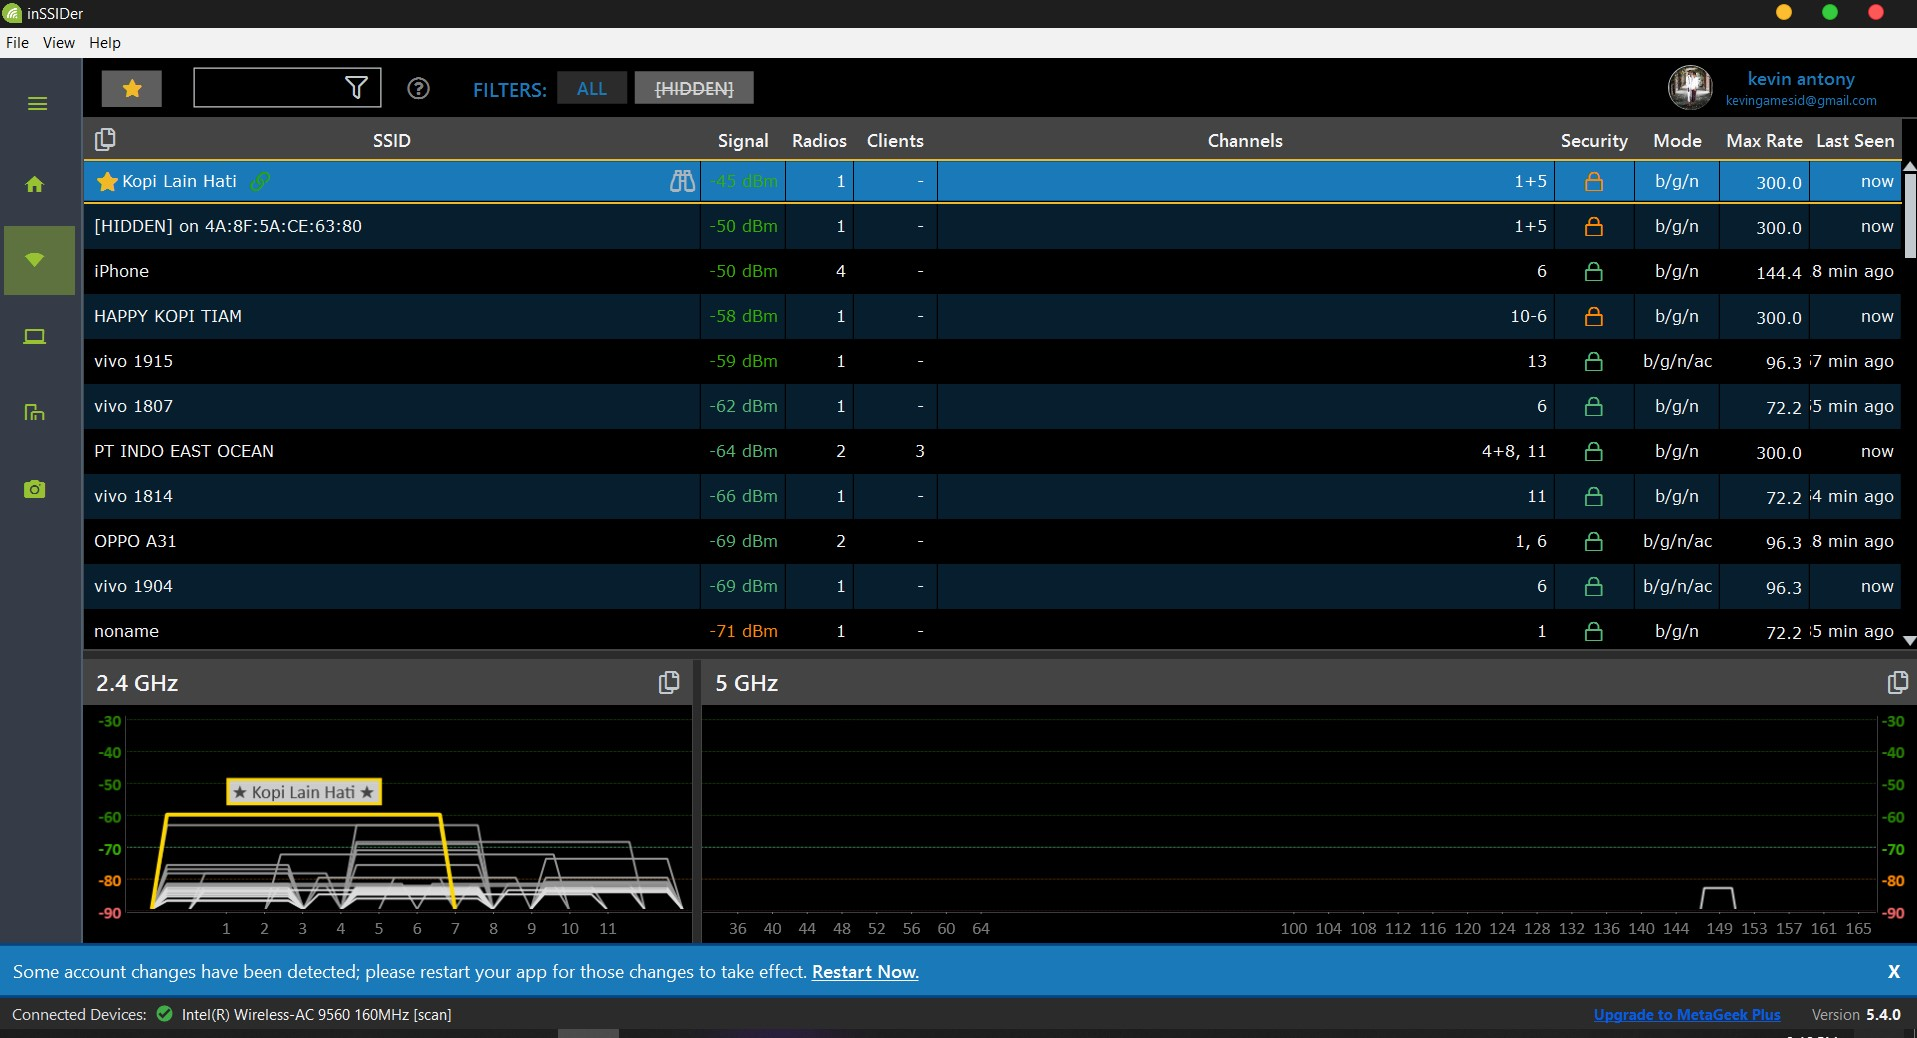
\includegraphics[width=.3\textwidth]{image/012.jpg}
     \caption{jarak 30 M}
     \end{figure}
     \vspace{4 cm}
     
\begin{itemize}
    \item Wifi 802.11 a/g
    \vspace{1pt}
    
    Standard IEEE 802.11a bekerja pada frekuensi 5 GHz mengikuti standard dari UNII (Unlicensed National Information Infrastructure). Teknologi IEEE 802.11a tidak menggunakan teknologi spread-spectrum melainkan menggunakan standar frequency division multiplexing (FDM). Mampu mentransfer data hingga 54 Mbps
    
\end{itemize}

\bibliographystyle{IEEEtran}
\cite{DhaniPro2021}
\cite{IlmuKomputer.com2021}
\cite{Khayat2012}
\cite{Kreasi2021}
\cite{Metageek2021}
\bibliography{IEEEabrv,refeerences.bib}


\end{document}
